\documentclass[12pt,a4paper]{article}
\usepackage[german]{babel}
\usepackage[T1]{fontenc}
\usepackage[utf8x]{inputenc}
\usepackage{url}
\usepackage{graphicx}
\usepackage{algpseudocode}
\usepackage{algorithm}
\usepackage{geometry}
\usepackage{amsfonts}
\usepackage{amsmath}
\usepackage{tabularx}
\usepackage{txfonts} %Times New Roman Font
\usepackage{titlesec} %Format der Headings ändern
\usepackage{hyperref}
\usepackage{comment}
\usepackage{listings}
\usepackage{pythonhighlight}

\renewcommand{\thesection}{\arabic{section}.} %Nummerierung der Sections anpassen
\renewcommand{\labelenumi}{\alph{enumi})}  %Nummerierung der Listen anpassen
\titleformat{\section}{\large\bfseries}{\thesection}{0.5em}{} %Format der Section Überschrift ändern
\setlength{\parindent}{0pt} %Keine Einrückung bei neuen Paragraphen
\geometry{left=2.0cm,textwidth=17cm,top=2.5cm,textheight=23cm}

% Anpassen %
%%%%%%%%%%%%%%%%%%%%%%%%%%%%%%%%%%%%%
\newcommand{\student}{Daniel Pantjuskin-Moos\\ 108013248222 } % Namen eintragen
\newcommand{\partner}{Vincent König\\ 108011232630} % Matrikelnummer eintragen
\newcommand{\group}{D} % Gruppennummer eintragen
%%%%%%%%%%%%%%%%%%%%%%%%%%%%%%%%%%%%%

\newcommand{\hwheadtwo}{$ $
  \vspace{-2cm}
  
\noindent \student \qquad \qquad  Wireless Physical Layer Security Praktikum \hfill SS 2020 \\
\noindent \partner \\
%\noindent \thirdone \\  % einkommentieren, falls ihr eine 3er Gruppe seid
\noindent Gruppe:~\group\\
$ $

  
\begin{center}    
{\Large \bf Abgabe PHYSEC 3}
\end{center}
}

\begin{document}
\hwheadtwo

\section{Messungen}

\section{Implementierung Pearson Correlation}


Die Aufgabenstellung ist, die in Abbildung~\ref{fig:Label1}
abgebildete Formel in einem vorgegeben Python-Code als 
Funktion \textit{correlation(X, Y)} zu implementieren, sodass 
es von einem mitgegeben Framework fehlerlos getestet werden 
kann. Die vollständige \textit{exercise3.py} kann  
\href{https://mega.nz/file/7gwx0BwR#dwkLdHX7AglZKYwp9poGQ-tEL20GtaqFy8LoT4TtV_g}
{hier} 
heruntergeladen werden.

\begin{figure}[hbt!]
	\centering
		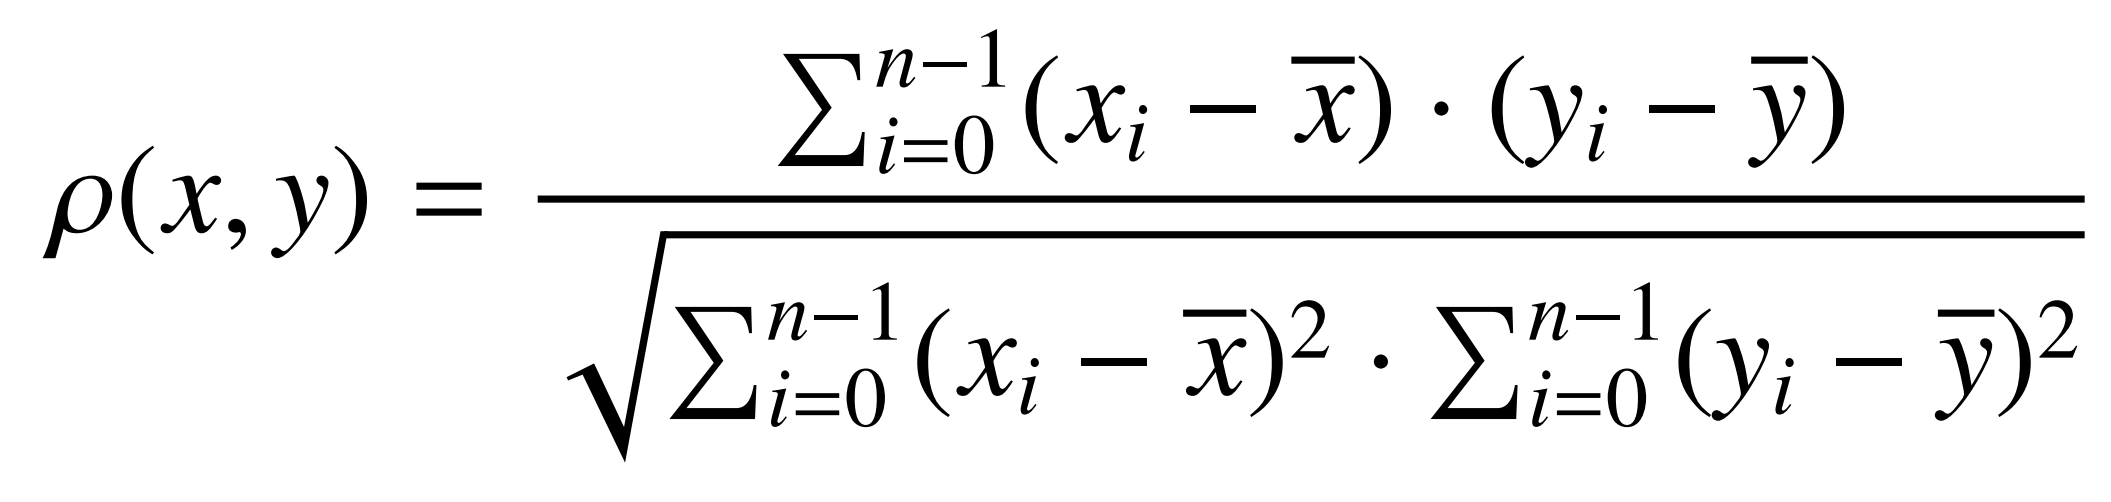
\includegraphics[width=0.8\textwidth ]
		{Bilder/a2-pearson-formel.png}
		\caption{Auszug aus dem Assignment}
		\label{fig:Label1}
\end{figure}
\newpage
\begin{python}

import utils
import numpy

"""
Excersise 3:
Implement the Pearson correlation coefficient.
Do NOT use any given function for standard-deviation 
or mean-value but implement them by yourself.

X, Y are given as lists.

Blockwise application is done outside so please use the 
whole vectors at once.
"""


def correlation(X, Y):
    mean_x = numpy.mean(X) # Mittel Vektor X
    mean_y = numpy.mean(Y) # Mittel Vektor Y

    numerator = 0 # zaehler
    denominator_x = 0 # der X beinhaltene Faktor im Nenner
    denominator_y = 0 # der Y beinhaltene Faktor im Nenner

    # Falls Vektoren unterschiedlich lang sind
    if len(X) != len(Y):
        raise Exception("Length not equal!\n")

    for i in range(len(X)):
        numerator += (X[i] - mean_x)*(Y[i] - mean_y)
        denominator_x += (X[i]-mean_x)*(X[i]-mean_x)
        denominator_y += (Y[i]-mean_y)*(Y[i]-mean_y)

    denominator = numpy.sqrt(denominator_x * denominator_y)

    # Falls Nenner=0, dann wird der jeweilige Eintrag ignoriert
    # und wird somit auch nicht in die Skizzen eingetragen
    if denominator == 0:
        return float('nan')

    pearson = numerator/denominator

    return pearson
    # return utils.not_yet_implemented("Correlation")

\end{python}


\newpage
\section{Auswertung}

Die Messproben wurden mit 74 verschiedenen Tests analysiert. 
Die Testergebnisse und die dazugehörigen Befehle können 
\href{https://mega.nz/file/rg4HzTJB#4DSJFln2TZiz9BZ_8xZObXRsGiheQ3Otaf_7wMUAqTQ}
{hier} 
heruntergeladen werden. Zuerst beschreiben mit römischen 
Zahlen nummerierte Abschnitte, welche Auffälligkeiten die 
dazugehörigen Teilaufgaben aus Aufgabe 1 aufweisen. Danach 
werden die allgemeinen Fragen aus der Aufgabenstellung zu 
Aufgabe 3 beantwortet.


\subsection*{Hinweis zu Mittel und Median}

Alle Werte werden ignoriert bei denen die Nenner bei der 
Berechnung der Pearson Korrelationen gleich Null sind. 
Bei der Bestimmung der Mittel und Mediane wurden von allen 
Korrelationen die Beträge gebildet. Es wird auf vier 
Nachkommastellen gerundet. In der \textit{correlation(X,Y)}
werden diese Fälle mit \textit{nan} vermerkt, welche dann 
in den Skizzen ausgelassen werden.


\subsection*{\textit{i)}}


Alice sendet an Bob :\\~\\


\Large
\begin{tabular}{ |p{3cm}|||p{3cm}|p{3cm}||p{3cm}|p{3cm}|}
    \hline
    \multicolumn{5}{|c|}{Teilaufgabe 1: $A\rightarrow B$} \\
    \hline
    Blockgröße & Mittel Bob & Median Bob & Mittel Eve & Median Eve\\
    \hline
    \hspace{3.2mm}30 & 0.2290 & 0.1756 & 0.1798 & 0.1428\\
    100 & 0.2219 & 0.1848 & 0.1341 & 0.1053\\
    200 & 0.2401 & 0.2377 & 0.0946 & 0.0748\\
    250 & 0.2591 & 0.2328 & 0.1495 & 0.1260\\
    300 & 0.2791 & 0.2108 & 0.1784 & 0.1130\\
    \hline
\end{tabular}
\\[0.7cm]\\
\normalsize

Es fällt auf, dass mit zunehmender Blockgröße weniger Nullen in den 
Nennern auftreten. Bob hat wie zu erwarten, durchgehend größere 
Korrelationen. Außerdem steigen Bobs Korrelationen in dieser Messung 
mit der Blockgröße bis mindestens 300. Eves Korrelationen weisen
bei den verwendeten Blockgrößen eine negativen Buckel auf, mit 
Tiefpunkt bei Blockgröße 200. Interessant ist auch, dass bei 
Blockgröße 250 (und 300), der erste Eintrag deutlich höher liegt 
als die anderen, siehe Abbildungen~\ref{fig:Label2} bis 
~\ref{fig:Label5}. Außerdem zeichnet sich 
der Trend ab, dass Eve deutlich mehr negative Korrelationen hat.

\begin{figure}[hbt!]
	\centering
		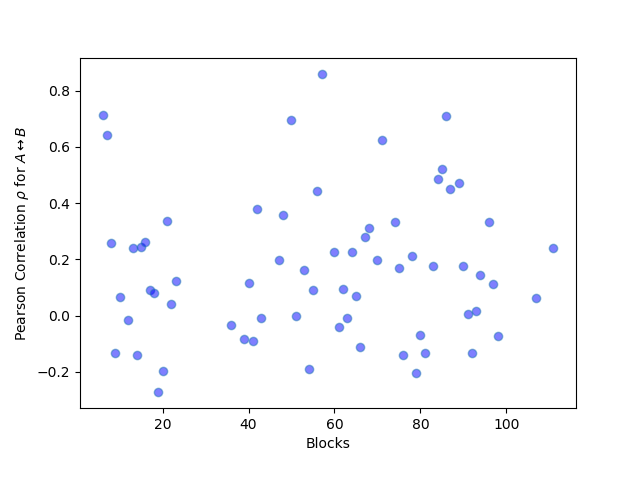
\includegraphics[width=0.75\textwidth ]
		{Bilder/a3-t1-block30-correlation-AB.png}
		\caption{Skizze der Korrelation zwischen A und B mit Blockgröße 30}
		\label{fig:Label2}
\end{figure}

\begin{figure}[hbt!]
	\centering
		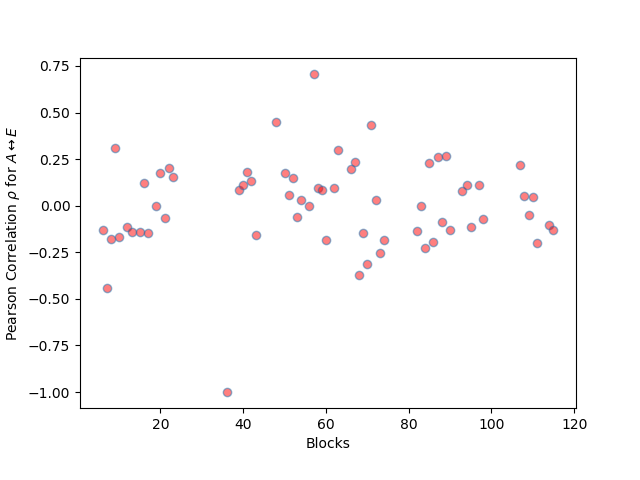
\includegraphics[width=0.75\textwidth ]
		{Bilder/a3-t1-block30-correlation-AE.png}
		\caption{Skizze der Korrelation zwischen A und E mit Blockgröße 30}
		\label{fig:Label3}
\end{figure}
\clearpage


\begin{figure}[hbt!]
	\centering
		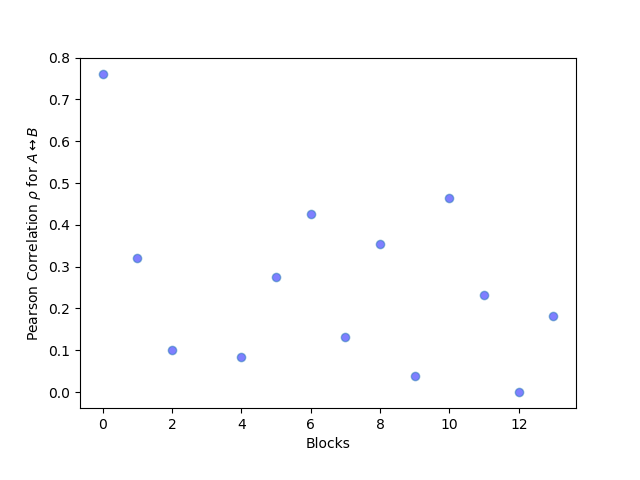
\includegraphics[width=0.75\textwidth ]
		{Bilder/a3-t1-block250-correlation-AB.png}
		\caption{Skizze der Korrelation zwischen A und B mit Blockgröße 250}
		\label{fig:Label4}
\end{figure}

\begin{figure}[hbt!]
	\centering
		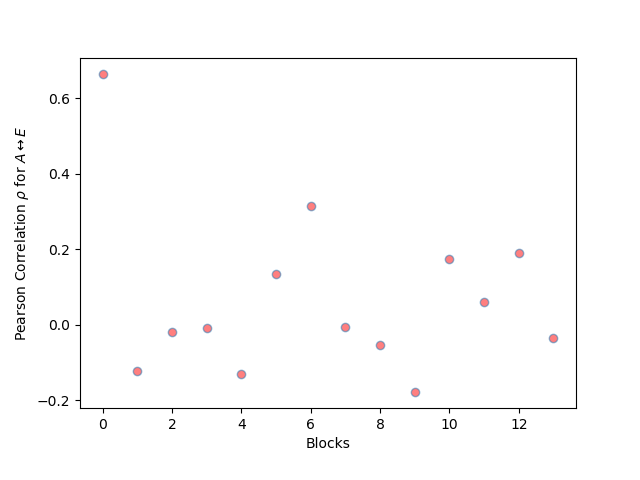
\includegraphics[width=0.75\textwidth ]
		{Bilder/a3-t1-block250-correlation-AE.png}
		\caption{Skizze der Korrelation zwischen A und E mit Blockgröße 250}
		\label{fig:Label5}
\end{figure}
\clearpage

\subsection*{\textit{ii)}}


Alice sendet an Bob, aber diesmal wird für Bewegung 
zwischen den Knoten gesorgt:\\~\\


\Large
\begin{tabular}{ |p{3cm}|||p{3cm}|p{3cm}||p{3cm}|p{3cm}|}
    \hline
    \multicolumn{5}{|c|}
    {Teilaufgabe 1: $A\rightarrow B$ mit Bewegung zischen den Knoten}\\
    \hline
    Blockgröße & Mittel Bob & Median Bob & Mittel Eve & Median Eve\\
    \hline
    \hspace{3.2mm}30 & 0.9807 & 0.9901 & 0.2522 & 0.2626\\
    
    200 & 0.9912 & 0.9925 & 0.2365 & 0.2337\\
   
    300 & 0.9918 & 0.9932 & 0.2339 & 0.2495\\
    \hline
\end{tabular}
\\[0.7cm]\\
\normalsize

\begin{figure}[hbt!]
	\centering
		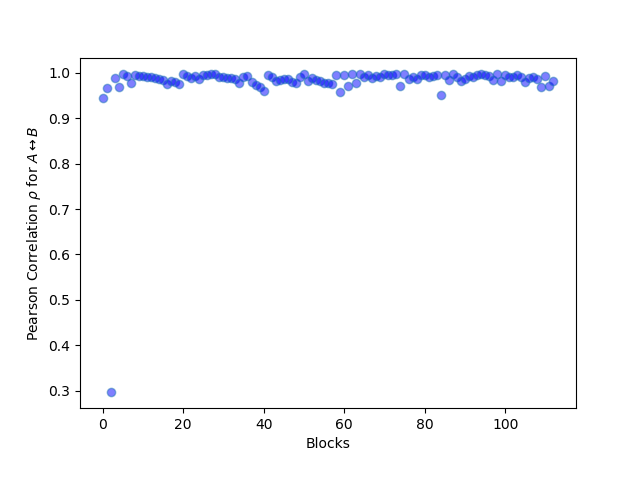
\includegraphics[width=0.75\textwidth ]
		{Bilder/a3-t2-block30-correlation-AB.png}
		\caption{Skizze der Korrelation zwischen A und B mit Blockgröße 30 (mit Bewegung)}
		\label{fig:Label6}
\end{figure}

\begin{figure}[hbt!]
	\centering
		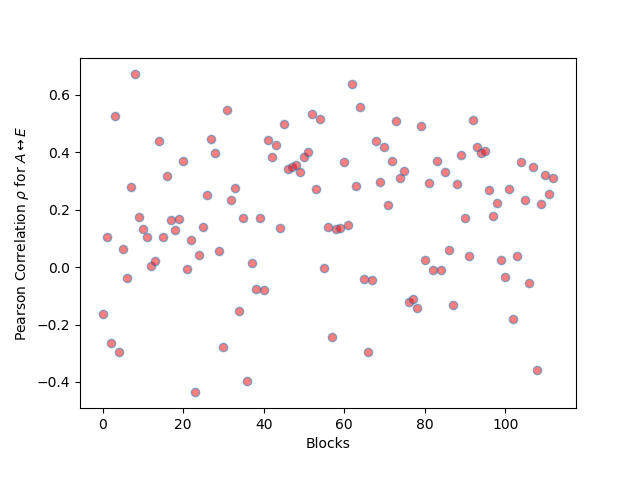
\includegraphics[width=0.75\textwidth ]
		{Bilder/a3-t2-block30-correlation-AE.png}
		\caption{Skizze der Korrelation zwischen A und E mit Blockgröße 30 (mit Bewegung)}
		\label{fig:Label7}
\end{figure}



Auffallend ist, dass der Unterschied nun ohne Probleme mit dem bloßen 
Auge klar zu erkennen ist. Bobs Korrelationen sind fast durchgehend der 
eins sehr nahe, wobei Eves Korrelationen besser sind als zuvor und 
zunehmend mit der Blockgröße seltener im negativen Bereich, aber dennoch
weit abgeschlagen hinter Bobs Korrelationen.


\subsection*{\textit{iii)}: Keine Bewegung}


Es treten sehr oft nullen in den Nennern auf die dann mit 
\textit{nan} gekennzeichnet wurden. Wie zu erwarten war, gab 
es mit Abstand etwa 20cm deutlich mehr von diesen Fällen. 
Bei Bob war sogar bei 20cm jedes einzelne Ergebnis wie 
zum Beispiel in Abbildung~\ref{fig:Label8} erkennbar \textit{nan}
was zur Folge hat, dass diese skizze leer ist. 
Umgekehrt gibt es bei plus 10m Abstand deutlich weniger
\textit{nan}-Fälle. Bob hat da keine einzige leere Skizze.
Insgesamt ist die Korrelation bei Bob und Eve klar höher.
Es lässt sich beobachten, dass das Mittel bei Eve +10m bei Blockgröße
30 mit 0.1686 deutlich größer ist als bei Blockgröße 300 mit 0.0467.

\newpage
\subsubsection*{Keine Bewegung (20cm)}


\begin{figure}[hbt!]
	\centering
		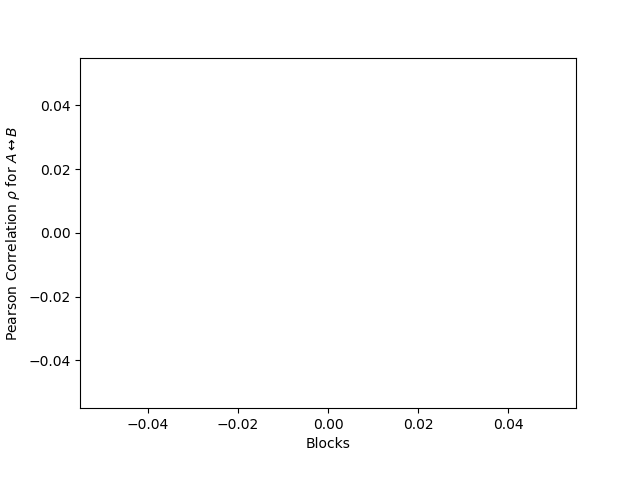
\includegraphics[width=0.7\textwidth ]
		{Bilder/a3-t3a-ob-block100-correlation-AB.png}
		\caption{Skizze der Korrelation zwischen A und B mit Blockgröße 100 (20cm)}
		\label{fig:Label8}
\end{figure}

\begin{figure}[hbt!]
	\centering
		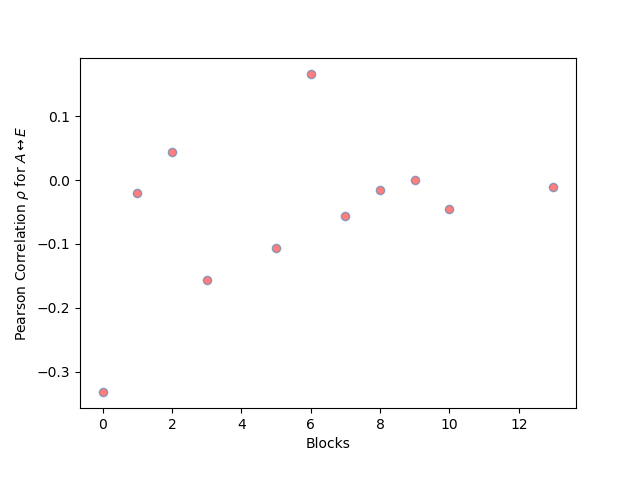
\includegraphics[width=0.7\textwidth ]
		{Bilder/a3-t3a-ob-block100-correlation-AE.png}
		\caption{Skizze der Korrelation zwischen A und E mit Blockgröße 100 (20cm)}
		\label{fig:Label9}
\end{figure}
\clearpage



\subsubsection*{Keine Bewegung (+10m)}

\begin{figure}[hbt!]
	\centering
		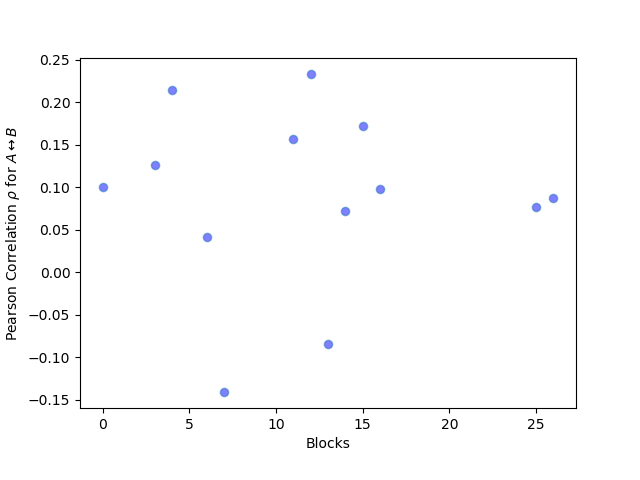
\includegraphics[width=0.7\textwidth ]
		{Bilder/a3-t3b-ob-block100-correlation-AB.png}
		\caption{Skizze der Korrelation zwischen A und B mit Blockgröße 100 (+10m)}
		\label{fig:Label10}
\end{figure}

\begin{figure}[hbt!]
	\centering
		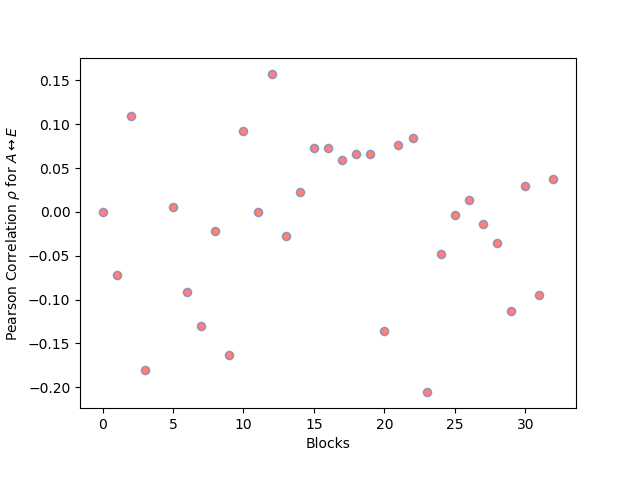
\includegraphics[width=0.7\textwidth ]
		{Bilder/a3-t3b-ob-block100-correlation-AE.png}
		\caption{Skizze der Korrelation zwischen A und E mit Blockgröße 100 (+10m)}
		\label{fig:Label11}
\end{figure}
\clearpage






\subsection*{\textit{iii)}: Mit Bewegung}

Wie zu erwarten war, sind hier die Korrelationen im 
Vergleich zu den Abbildungen~\ref{fig:Label8} bis
~\ref{fig:Label11} deutlich größer. Die Korrelation bei 
Bob ist bei +10m ein bisschen kleiner, bei Eve jedoch ist 
die Korrelation bei +10m sehr deutlich größer. Reichten die 
Korrelationen bei Eve bei 20cm von etwa -0.4 bis 0.3 so 
reichen sie bei +10m von etwa 0.3 bis 0.8 siehe Abbildungen
~\ref{fig:Label13} und ~\ref{fig:Label15} 



\subsubsection*{Mit Bewegung (20cm)}


\begin{figure}[hbt!]
	\centering
		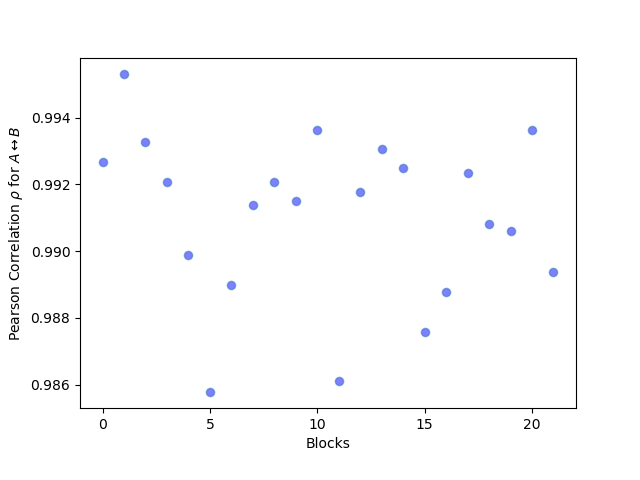
\includegraphics[width=0.6\textwidth ]
		{Bilder/a3-t3a-mb-block100-correlation-AB.png}
		\caption{Skizze der Korrelation zwischen A und B mit Blockgröße 100 (20cm) mit Bewegung}
		\label{fig:Label12}
\end{figure}

\begin{figure}[hbt!]
	\centering
		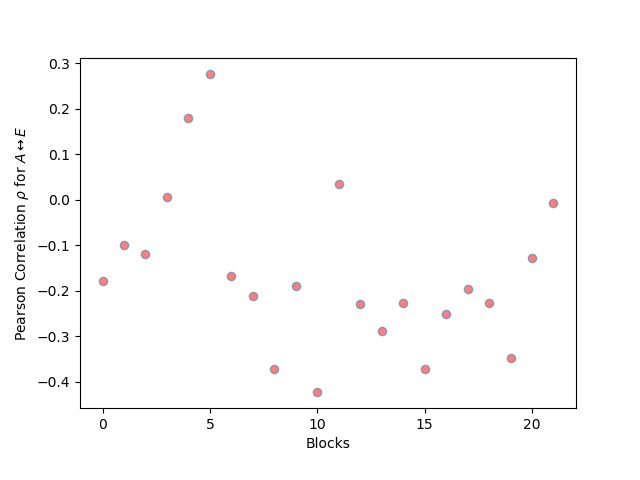
\includegraphics[width=0.6\textwidth ]
		{Bilder/a3-t3a-mb-block100-correlation-AE.png}
		\caption{Skizze der Korrelation zwischen A und E mit Blockgröße 100 (20cm) mit Bewegung}
		\label{fig:Label13}
\end{figure}
\clearpage



\subsubsection*{Mit Bewegung (+10m)}


\begin{figure}[hbt!]
	\centering
		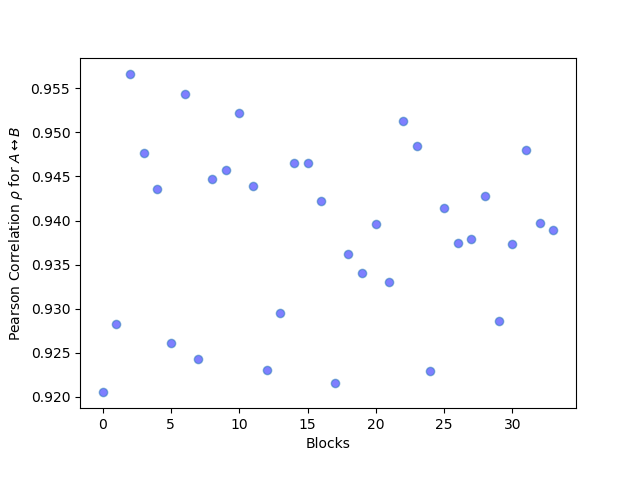
\includegraphics[width=0.7\textwidth ]
		{Bilder/a3-t3b-mb-block100-correlation-AB.png}
		\caption{Skizze der Korrelation zwischen A und B mit Blockgröße 100 (+10m) mit Bewegung}
		\label{fig:Label14}
\end{figure}

\begin{figure}[hbt!]
	\centering
		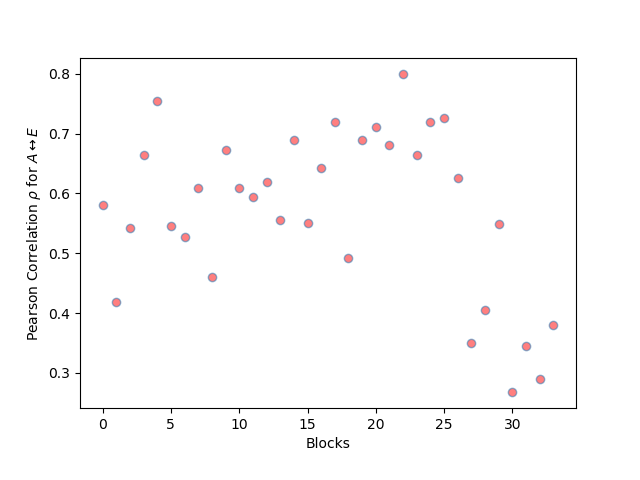
\includegraphics[width=0.7\textwidth ]
		{Bilder/a3-t3b-mb-block100-correlation-AE.png}
		\caption{Skizze der Korrelation zwischen A und E mit Blockgröße 100 (+10m) mit Bewegung}
		\label{fig:Label15}
\end{figure}


\subsection*{\textit{iv)}}

Knoten A wird bei diesen Messungen manuel bewegt. Die Ergebnisse
sind mit denen von Unterabschnitt \textit{ii)} zu vergleichen mit 
einem Mittel bei Bob bei Blockgröße 300 von etwa 0.9946 
beziehungsweise 0.2696 bei Eve (etwa besser).

\begin{figure}[hbt!]
	\centering
		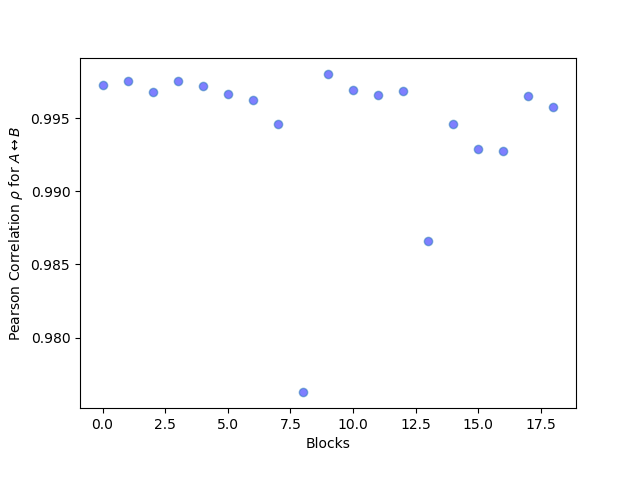
\includegraphics[width=0.62\textwidth ]
		{Bilder/a3-t4-block300-correlation-AB.png}
		\caption{Skizze der Korrelation zwischen A und B mit Blockgröße 300 mit manueller Bewegung von Knoten A}
		\label{fig:Label16}
\end{figure}

\begin{figure}[hbt!]
	\centering
		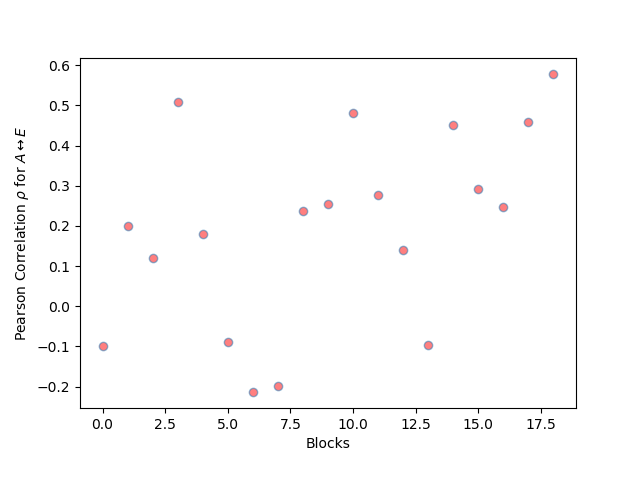
\includegraphics[width=0.62\textwidth ]
		{Bilder/a3-t4-block300-correlation-AE.png}
		\caption{Skizze der Korrelation zwischen A und E mit Blockgröße 300 mit manueller Bewegung von Knoten A}
		\label{fig:Label17}
\end{figure}
\clearpage




\subsection*{\textit{v)}}
Wie \textit{v)}, aber mit Knoten E sehr nahe an B ohne sich 
gegenseitig zu berühren.


\begin{figure}[hbt!]
	\centering
		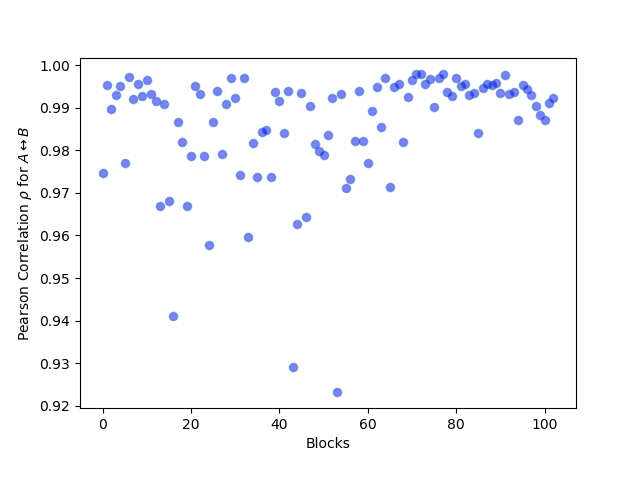
\includegraphics[width=0.62\textwidth ]
		{Bilder/a3-t5-block30-correlation-AB.png}
		\caption{Skizze der Korrelation zwischen A und B mit Blockgröße 30 mit manueller Bewegung von Knoten A und E sehr nahe an B}
		\label{fig:Label18}
\end{figure}

\begin{figure}[hbt!]
	\centering
		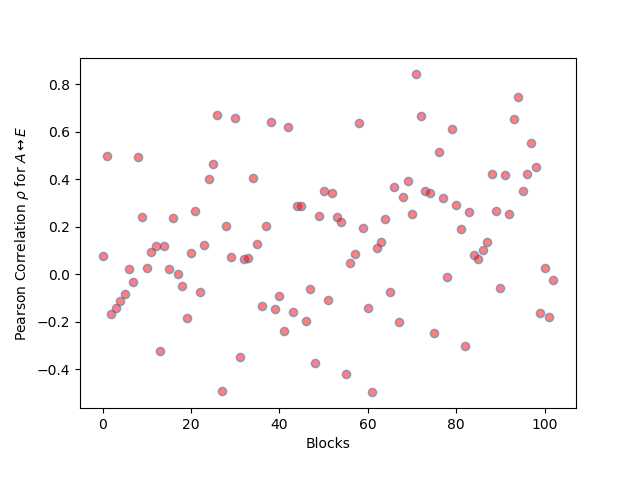
\includegraphics[width=0.62\textwidth ]
		{Bilder/a3-t5-block30-correlation-AE.png}
		\caption{Skizze der Korrelation zwischen A und B mit Blockgröße 30 mit manueller Bewegung von Knoten A und E sehr nahe an B}
		\label{fig:Label19}
\end{figure}
\clearpage


\begin{figure}[hbt!]
	\centering
		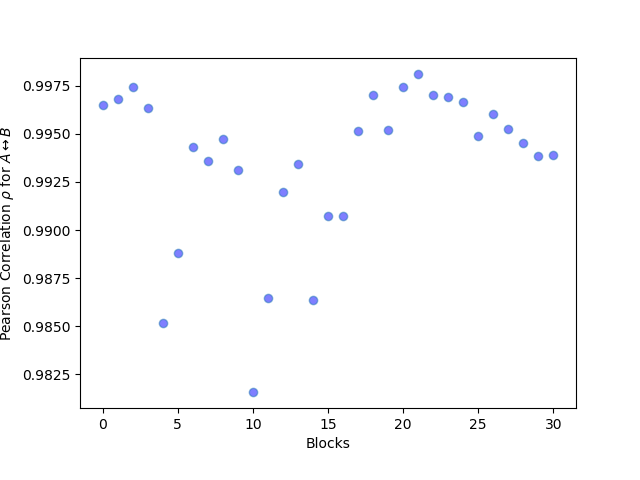
\includegraphics[width=0.62\textwidth ]
		{Bilder/a3-t5-block100-correlation-AB.png}
		\caption{Skizze der Korrelation zwischen A und B mit Blockgröße 100 mit manueller Bewegung von Knoten A und E sehr nahe an B}
		\label{fig:Label20}
\end{figure}

\begin{figure}[hbt!]
	\centering
		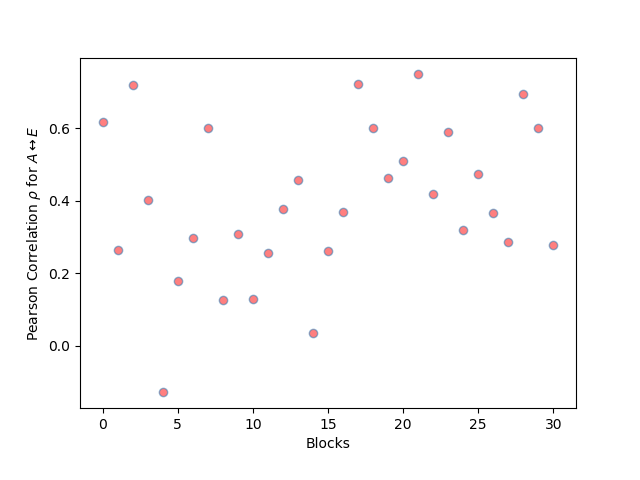
\includegraphics[width=0.62\textwidth ]
		{Bilder/a3-t5-block100-correlation-AE.png}
		\caption{Skizze der Korrelation zwischen A und B mit Blockgröße 100 mit manueller Bewegung von Knoten A und E sehr nahe an B}
		\label{fig:Label21}
\end{figure}
\clearpage

\begin{figure}[hbt!]
	\centering
		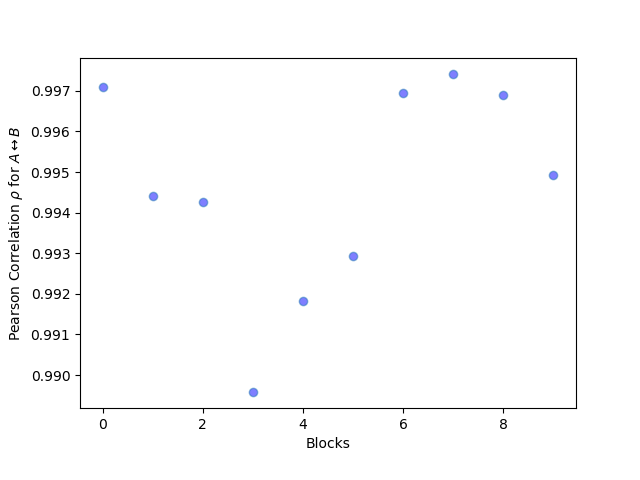
\includegraphics[width=0.62\textwidth ]
		{Bilder/a3-t5-block300-correlation-AB.png}
		\caption{Skizze der Korrelation zwischen A und B mit Blockgröße 300 mit manueller Bewegung von Knoten A und E sehr nahe an B}
		\label{fig:Label22}
\end{figure}

\begin{figure}[hbt!]
	\centering
		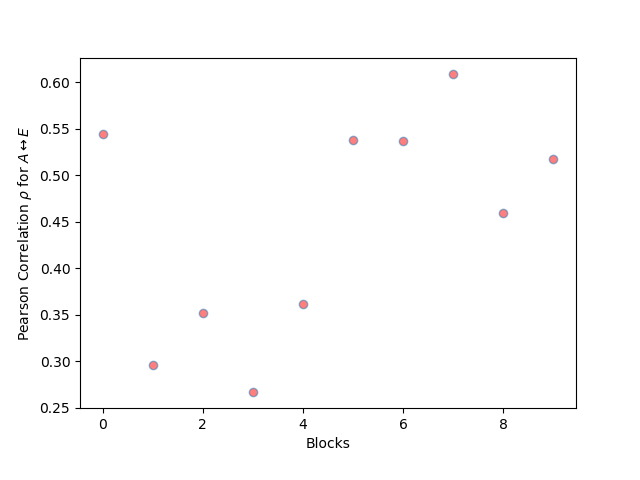
\includegraphics[width=0.62\textwidth ]
		{Bilder/a3-t5-block300-correlation-AE.png}
		\caption{Skizze der Korrelation zwischen A und B mit Blockgröße 300 mit manueller Bewegung von Knoten A und E sehr nahe an B}
		\label{fig:Label23}
\end{figure}


Bob hat durchgehend eine große Korrelation von
etwa 0.99, egal ob Blockgröße 30 oder 300. Bei Eve zeichnet sich ein 
anderes Verhalten ab, siehe Abbildungen~\ref{fig:Label19},~\ref{fig:Label21},
~\ref{fig:Label23}. So ist das Mittel bei Eve bei Blockgröße 30, selbst 
wenn man die Beträge von den vielen negativen Werten miteinbezieht, nur 
bei 0.2596. Bei Blockgröße 300 allerdings ist es 0.4482.


\newpage
\section{Quantisierer Jana Multibit}
\subsection*{a) Funktionsweise}
Alice und Bob sammeln RSS Messungen und bestimmen den Bereich der gemessenen Werte(Range of RSS). Anschließend wird \textit{N}, eine Nummer, wieviele Bits pro Messung extrahiert werden können, bestimmt. Danach werden die Messungen in $M = 2^N$ gleich große Intervalle unterteilt. Für jedes dieser Intervalle wird eine N-Bit Zuordnung gewählt. Liegt die Messung nun im Intervall, so wird sie dem \textit{Bitstream} hinzugefügt. Andernfalls muss sie erst korrigiert werden.

\subsection*{b) Pseudocode}
\begin{algorithm}
\caption{Pseudocode}
\begin{algorithmic}[1]
\State $range = max[RSS] - min[RSS]$
\State $N \in [0, log_2 RSS]$
\State $M = 2^N$
\State $RSS[] \to M$ intervalls $I[]$ of equal size
\State Choose $N$ bit assignment $\forall$ $M$ intervalls
\For{$t \to len(RSS[])$}
\For{$i \to len(I[]$}
\If{$RSS[t] \in I[i]$}
\State $bitstream \gets$ bit assignment
\EndIf
\EndFor
\EndFor\\
\Return $bitstream$
\end{algorithmic}
\end{algorithm}

\newpage
\section{Quantisierer Mathur Suhas}
\subsection*{a) Funktionsweise}
Bob und Alice haben beide die gleiche Anzahl an Schätzwerten $h_a$ und $h_b$.\\
$h_a(j)$ sowie $h_b(j)$ korrespondieren jeweils $\forall j \in [1,len(h_a)]$.\\
Alice wählt zufällige m-elementige Teilmenge die unter $q_-$ oder über $q_+$ liegt und speichert diese Messungen in einer Liste L ab. Diese Liste wird nun an Bob gesendet.\\
Bob überprüft nun für jeden Eintrag der Liste, ob seine Messungen $h_b$ korrekt sind. Jeder Eintrag der nicht übereinstimmt wird in eine Liste L' eingetragen. Diese Liste wird dann an Alice zurückgesendet.\\
Nun können beide mit Hilfe der Liste L' $Q(h_a)$ bzw. $Q(h_+)$ berechnen.

\subsection*{b) Pseudecode}
\begin{algorithm}
\caption{Pseudocode}
\begin{algorithmic}[1]
\State Alice creates List L
\State Alice sends L $\to$ Bob
\State Bob compares L to his List
\State Bob creates List L'
\State Bob sends L' $\to$ Alice
\State Alice and Bobo generate mutual Bitstream
\end{algorithmic}
\end{algorithm}

\newpage
\section{Bonus: Reading Assignment}
\subsection*{a)}
Die Autoren sind auf der Suche nach nach einem effizienten und sicheren Algorithmus. Dieser soll den kabellosen Kanal möglichst effizient nutzen und soll Nutzerfreundlich sein, indem er z.b. einen sicheren Schlüssel in kurzer Zeit generieren kann.

\subsection*{b)}
Es ist eminent, dass der Probing-Algorithmus sich den Kanaleigenschaften anpassen kann, da der \textit{probing process} ansonsten nicht effizient sein kann, wenn der Kanal sich nicht ändert. Das kann bspw. passieren, wenn keine Informationen oder redundate Informationen immer wieder gesendet werden.



\begin{comment}
% Beispiel für einen Hyperlink 	
\href{https://www.rub.de}{hier klicken}

% Beispiel für Bilder mit Caption und Referenz

\begin{figure}[hbt!]
	\centering
		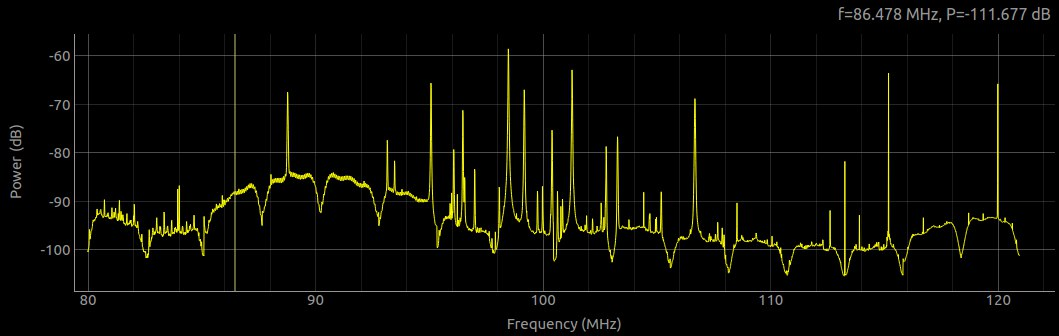
\includegraphics[width=1\textwidth ]
		{Bilder/a3_rtl_sdr.jpg}
		\caption{Hier Caption einfügen}
		\label{fig:Labelx}
\end{figure}

% Als Beispiel wie man referenziert
~\ref{fig:Labelx}

% Beispiel für das Einfügen von Python Code
\begin{python}
print("Hello World")
\end{python}

% Beispiel für das Erzwingen von Abstand 
\hspace{0.5mm}

\end{comment}

\end{document}